% =====================================================================
% ACVR 2026 (ECCV 2026 workshop) submission — ANONYMIZED (double-blind)
% PORTABLE PREAMBLE: this compiles as `article` on Overleaf as-is so you
% can preview. For the real submission, download the ECCV 2026 Author Kit
% and REPLACE the preamble (between the two ==== lines) with the kit's
% \documentclass[review]{eccv} (or llncs) preamble; the BODY is unchanged.
% Page limit: 14 pp excluding references. Keep it tight/academic.
% =====================================================================
\documentclass[10pt,twocolumn]{article}
\usepackage[T1]{fontenc}
\usepackage[utf8]{inputenc}
\usepackage[margin=19mm]{geometry}
\usepackage{amsmath,amssymb}
\usepackage{booktabs}
\usepackage{graphicx}
\usepackage{xcolor}
\usepackage{tikz}
\usetikzlibrary{arrows.meta,positioning}
\usepackage[hidelinks]{hyperref}
\usepackage{caption}
\captionsetup{font=small,labelfont=bf}
\newcommand{\todo}[1]{\textcolor{red}{[#1]}}
\newcommand{\code}[1]{\texttt{\small #1}}
\pagestyle{plain}
% =====================================================================

\title{\vspace{-8mm}\textbf{Drop-to-Annotate: Browser-Integrated Sign Segmentation
and Open-Vocabulary Gloss Spotting for Assistive Sign-Language Annotation}}
\author{Anonymous ACVR 2026 submission\\ \small Paper ID ****}
\date{}

\begin{document}
\maketitle

\begin{abstract}
Building large sign-language corpora is bottlenecked not by recording but by
\emph{annotation}: continuous signing must be cut into individual signs and each sign
labelled with a gloss tied to a lexical database. We present a browser-based,
human-in-the-loop annotation tool that embeds two neural models directly in the editing
loop so that dropping a video pre-populates the timeline with predicted sign boundaries and
each segment with a ranked list of candidate glosses; the annotator verifies and corrects
rather than authoring from scratch. Both models are \emph{RGB-only} (no pose extraction at
runtime): a frozen V-JEPA~2 video backbone with a lightweight recurrent (BiLSTM) frame-tagging
head for segmentation, and a self-supervised sign representation (Hiera-based) matched against
an open-vocabulary gloss dictionary by nearest-neighbour retrieval for spotting. To enable a
fair, \emph{reproducible} comparison we introduce a public benchmark built on the openly
available ECHO Sign Language of the Netherlands (NGT) corpus and evaluate our models against
external baselines (a pose-based linguistically-motivated segmenter, a hand-centric segmenter,
and a toolkit segmenter/spotter) under a single boundary-F1 / top-$k$ protocol. On in-domain
data our segmenter reaches a boundary F1 of \textbf{0.871}; on the cross-corpus ECHO benchmark
we report a striking result: a model trained only on Dutch/German signing under-segments badly
(boundary F1 0.13), but adding a \emph{different} sign language to training (Flemish, VGT) lifts it
to 0.25--0.35 RGB-only, matching pose-based zero-shot baselines. We release the benchmark annotations, splits, and
evaluation code (the corpus is fetched by users under its own licence).
\end{abstract}

\section{Introduction}
Sign-language datasets underpin recognition, translation, and linguistic research, yet they
are expensive to build: raw video must be temporally \emph{segmented} into individual signs and
each sign assigned a \emph{gloss} linked to a lexicon. Both steps are slow, repetitive, and
typically performed in desktop annotation software, frame by frame. This is an assistive,
human-in-the-loop problem: rather than fully automating annotation (where errors are costly and
trust is low), the goal is to \emph{accelerate the annotator} by proposing boundaries and
candidate labels they can accept or correct.

We describe a single-page web tool that does exactly this. On dropping a clip, the timeline is
pre-filled with predicted sign segments and each segment is pre-annotated with its ten most
likely glosses; the annotator's task shifts from authoring to verification. Two design choices
make this practical. First, both models are \emph{RGB-only}: they consume the normalised clip
the browser already holds, removing a brittle and expensive pose-estimation stage. Second,
spotting is framed as open-vocabulary retrieval, so the lexicon grows by adding dictionary
entries without retraining.

Our contributions are: (i) a deployed, browser-integrated segment-then-spot pipeline usable
without leaving the page; (ii) a \emph{public, reproducible} sign-segmentation and
gloss-spotting benchmark on the openly available ECHO NGT corpus, with a single evaluation
protocol; and (iii) a comparison of our RGB-only models against external pose-based and
hand-centric baselines, situating their accuracy and exposing the cross-corpus gap.

\section{Related work}
\paragraph{Sign segmentation.}
Temporal segmentation of continuous signing has been approached with pose-based sequence models
and with linguistically motivated boundary cues~\cite{moryossef2023}; hand-centric
representations have also been used for sign-boundary detection~\cite{handson}. Action-segmentation
heads such as MS-TCN~\cite{mstcn} are common backends. In contrast to pose-based pipelines we use
a frozen general-purpose video backbone (V-JEPA~2~\cite{vjepa2}) directly on RGB.
\paragraph{Sign spotting and representation.}
Sign spotting via dictionary retrieval scales the vocabulary without per-class
training~\cite{momeni}. Self-supervised sign representations~\cite{signrep} built on hierarchical
video transformers~\cite{hiera} provide signer-robust embeddings; we adapt one by
supervised-contrastive fine-tuning and retrieve against a gloss dictionary.
\paragraph{Annotation tooling.}
Multi-tier sign-language annotation is dominated by desktop editors such as ELAN and iLex; recent
work adds machine assistance (automatic segmentation or recognition) mostly as offline, batch
preprocessing steps. We instead embed warm neural inference \emph{inside} a single-page web editor
as a drop-to-annotate loop, so segmentation and gloss proposals appear in the timeline the
annotator is already working in.

\section{System overview}
The browser client normalises every dropped video to 25\,fps, H.264, $\leq$1080p (an in-page
WebAssembly FFmpeg) and issues two HTTPS requests: one whole-clip \code{/segment} call and one
\code{/spot} call per detected segment. Neither model runs in the browser; each is a warm,
long-lived GPU inference service behind a reverse proxy (Fig.~\ref{fig:arch}). Segmentation runs
only when a clip arrives without annotations, so importing an existing transcript leaves the
human's work untouched; the spotter is also invoked when the annotator creates a segment by hand.
Warm latency is $\approx$1\,s per spotting call and a few seconds per whole-clip segmentation.

\begin{figure}[t]\centering
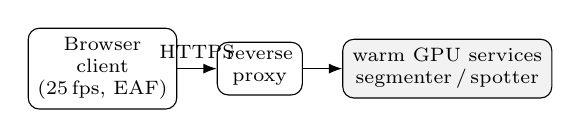
\begin{tikzpicture}[node distance=5mm,every node/.style={font=\scriptsize}]
\node[draw,rounded corners,align=center] (b){Browser\\client\\(25\,fps, EAF)};
\node[draw,rounded corners,right=of b,align=center](p){reverse\\proxy};
\node[draw,rounded corners,right=of p,align=center,fill=black!5](g){warm GPU services\\\,segmenter\,/\,spotter\,};
\draw[-{Latex}](b)--node[above]{HTTPS}(p);\draw[-{Latex}](p)--(g);
\end{tikzpicture}
\caption{The browser edits locally and calls two stateless HTTPS endpoints forwarded to warm
inference services that keep both models GPU-resident.}
\label{fig:arch}
\end{figure}

\section{Sign segmentation}
\paragraph{Frozen V-JEPA~2 backbone.}
Features come from V-JEPA~2~\cite{vjepa2}, a ViT-L video encoder pre-trained self-supervisedly on
general internet video, used \emph{frozen}. It is run on non-overlapping 16-frame chunks; patch
tokens are pooled to a $3\times3$ grid (nine region tokens of dimension 1024) per temporal
position. A \emph{phase-dual} scheme (two passes per chunk, one frame-shifted, interleaved) yields
one $9\times1024$ region-token vector per frame at 25\,Hz.
\paragraph{Recurrent region head and BIO decoding.}
A learned-query attention pool collapses the nine region tokens per frame to one vector; a
bidirectional LSTM then tags each frame with a BIO label (\code{OUT}/\code{IN}/\code{BEGIN}),
trained with a temporal-smoothing (T-MSE) loss. The served default \emph{ensembles} the BiLSTM
with an MS-TCN~\cite{mstcn} sibling by averaging per-frame label probabilities. Contiguous
non-\code{OUT} runs become \code{(start,end)} segments. The head is pre-trained on a German Sign
Language corpus and fine-tuned on an NGT sentence set, selecting the checkpoint by validation
boundary F1.

\section{Sign spotting}
A segment clip is encoded by a self-supervised sign representation~\cite{signrep} (Hiera
backbone~\cite{hiera}, masked-autoencoder pre-training with skeleton priors but \emph{no} keypoints
at inference) into a single 768-d embedding. We adapt it to NGT by supervised-contrastive
fine-tuning and, at serve time, \emph{ensemble} two fine-tuned backbones via per-segment
z-normalised score fusion. Each gloss in the lexicon has a pre-computed embedding; the query is
matched by cosine similarity and the ten nearest glosses are returned with scores. The deployed
dictionary holds 10{,}254 glosses, so any sign in the lexicon can in principle be proposed.

\section{The ECHO-NGT benchmark}
\label{sec:bench}
Prior numbers for systems like ours are typically reported on private data, preventing
comparison. We therefore define a reproducible benchmark on the \emph{openly available} ECHO NGT
corpus (Aesop fables, a lexicon elicitation, and poetry; 20 sessions, 25\,fps, five signers).
The corpus is distributed under CC BY-NC-ND; we release only \emph{derived annotations, split
definitions, and evaluation code}, with users fetching the media from the official archive.
\paragraph{Segmentation reference.} Ground-truth sign boundaries are the time-union of the
right- and left-hand gloss tiers, giving 2{,}904 sign segments. Because every method here is
trained on other corpora (DGS/CSL/NGT-sentences), \emph{all 20 sessions form a clean cross-corpus
test set}; we report boundary F1 at a fixed time tolerance, with a tolerance sweep.
\paragraph{Spotting set.} A self-dictionary of 2{,}936 exemplar clips over 884 glosses and 355
held-out query signs (216 covered by the dictionary); top-$k$ retrieval over covered queries. We
additionally report a signer-disjoint split (held-out signers) to test signer independence.
\paragraph{Baselines.} A pose-based linguistically-motivated segmenter~\cite{moryossef2023}
(DGS-trained, zero-shot on NGT), a hand-centric segmenter~\cite{handson} (zero-shot), a toolkit
pose segmenter, and a base (non-fine-tuned) retrieval spotter, all run through the same scorer.

\section{Results}
\paragraph{In-domain segmentation.} On the NGT sentence set (345 sentences, RGB, $\pm0.1$\,s
boundary tolerance) the served BiLSTM$\times$MS-TCN ensemble reaches boundary F1 \textbf{0.871}
(seg F1 0.800); a single BiLSTM reaches 0.817--0.848 by frame rate; MS-TCN alone 0.806
(Table~\ref{tab:seg-indomain}). Cross-lingual transfer to held-out DGS drops to 0.64--0.66.

\begin{table}[t]\centering\small
\caption{In-domain NGT-sentence segmentation (RGB, $\pm0.1$\,s).}
\label{tab:seg-indomain}
\begin{tabular}{lccc}\toprule
Head & fps & Bnd F1 & Seg F1\\\midrule
BiLSTM$\times$MS-TCN ens.\ (served) & 50 & \textbf{0.871} & \textbf{0.800}\\
BiLSTM & 50 & 0.848 & 0.750\\
BiLSTM & 25 & 0.817 & 0.750\\
MS-TCN & 25 & 0.806 & 0.739\\\bottomrule
\end{tabular}
\end{table}

\paragraph{ECHO benchmark — segmentation (cross-corpus).} Every segmenter here is applied
\emph{cross-corpus} to ECHO (trained on DGS/NGT-sentences or other languages, never on ECHO).
Table~\ref{tab:seg-echo} reports boundary F1 over all 20 sessions. Two things stand out. First,
\textbf{all methods collapse on recall} (boundary recall 0.09--0.17): the dominant failure is
\emph{missed} boundaries, not spurious ones. Second, our base RGB model is the most
\emph{conservative} — it has the highest boundary precision (0.33) but the lowest recall, so the
pose baselines obtain higher boundary F1 simply by proposing more segments. Adding a second sign
language to training (\textbf{+VGT}, Sec.~\ref{sec:multicorpus}) raises recall and closes most of
this gap, RGB-only, without any in-domain cost.

\begin{table}[t]\centering\small
\caption{ECHO-NGT segmentation (cross-corpus, boundary F1 @ $\pm0.1$\,s; 20 sessions, 2{,}904 ref.\ segments). Pose baselines are zero-shot; ours are RGB-only.}
\label{tab:seg-echo}
\begin{tabular}{lc}\toprule
Method & Bnd F1\\\midrule
Ours, V-JEPA~2 + BiLSTM (25\,fps) & 0.135\\
Ours, BiLSTM$\times$MS-TCN ensemble (50\,fps) & 0.105\\
\textbf{Ours + VGT (25\,fps, deployed)} & \textbf{0.254}\\
\midrule
Toolkit pose segmenter (zero-shot) & 0.193\\
Hand-centric (pose, zero-shot)~\cite{handson} & 0.263\\
Linguistically-motivated (pose, zero-shot)~\cite{moryossef2023} & 0.347\\
\bottomrule
\end{tabular}
\end{table}

\paragraph{Multi-corpus training closes the cross-corpus gap.}\label{sec:multicorpus}
We test whether adding out-of-domain corpora to pretraining repairs the cross-corpus deficit,
keeping the head/features/decoder fixed and varying only the pretrain pool (then finetuning on
NGT-Zin). Table~\ref{tab:multicorpus} evaluates each variant on in-domain NGT-Zin, on a
\emph{signer-disjoint} held-out ECHO split (BB+WE), and on held-out VGT. \textbf{Adding VGT
(a \emph{different} sign language) is the most effective fix}: it nearly doubles the
deployment-style (full-session) ECHO boundary F1 ($0.197\!\to\!0.347$) and moves the predicted
segment count to the reference, with no in-domain regression ($0.817\!\to\!0.813$). Adding ECHO
itself helps the windowed metric but degrades full-session stitching, and combining both gives
the best in-domain score but does not stack on ECHO. That a Flemish-SL corpus repairs Dutch-SL
cross-corpus segmentation is evidence the learned boundary cue is largely language-agnostic; the
\textbf{+VGT} model is the deployed configuration.

\begin{table}[t]\centering\small
\caption{Multi-corpus ablation (boundary F1 @ $\pm0.1$\,s). ECHO test is signer-disjoint (held-out BB+WE); window = 16\,s windows, sess = full-session (deployment-style).}
\label{tab:multicorpus}
\begin{tabular}{lcccc}\toprule
Pretrain pool & Zin & ECHO\,(win) & ECHO\,(sess) & VGT\\\midrule
DGS+NGT (baseline) & 0.817 & 0.231 & 0.197 & 0.469\\
\textbf{+\,VGT} & 0.813 & 0.315 & \textbf{0.347} & 0.405\\
+\,ECHO & 0.796 & \textbf{0.327} & 0.108 & 0.444\\
+\,VGT+ECHO & \textbf{0.826} & 0.320 & 0.096 & 0.359\\\bottomrule
\end{tabular}
\end{table}

\paragraph{Spotting.} On the in-domain NGT sentence bench the served two-backbone ensemble
reaches top-1 67.3 / top-5 87.2 with the deployed coverage dictionary (10{,}254 glosses) and
71.2 / 91.0 with the smaller accuracy dictionary (1{,}818 glosses; Table~\ref{tab:spot}). On the
held-out ECHO spotting set (216 covered queries) a base SignRep encoder scores top-1 0.139;
NGT-sentence fine-tuning is roughly neutral cross-corpus, while an ECHO-specific fine-tune gives a
small in-domain gain (top-1 0.148). As with segmentation, cross-corpus robustness tracks training
\emph{diversity} rather than in-domain specialisation.

\begin{table}[t]\centering\small
\caption{Sign spotting on the held-out NGT-sentence bench (249 sentences, lexical signs, exact match), two-backbone ensemble.}
\label{tab:spot}
\begin{tabular}{lccc}\toprule
Dictionary & Glosses & Top-1 & Top-5\\\midrule
Coverage (deployed) & 10{,}254 & 0.673 & 0.872\\
\textbf{Accuracy (best)} & 1{,}818 & \textbf{0.712} & \textbf{0.910}\\\bottomrule
\end{tabular}
\end{table}

\section{Ethics and reproducibility}
\paragraph{Data and consent.} All corpora used are research sign-language datasets recorded with
participant consent for research use. ECHO is distributed under CC~BY-NC-ND; we therefore release
only \emph{derived} annotations (boundary tables, split definitions) and evaluation code, and never
redistribute its video or modified annotations --- users obtain the media from the official
archive. Sign-language video shows identifiable signers; this system is intended as an assistive
annotation aid, not for identification or surveillance.

\paragraph{Reproducibility.} The segmentation head is a small BiLSTM (with an optional MS-TCN
sibling) over \emph{frozen} V-JEPA~2 features, trained with AdamW (pretrain lr $3\!\times\!10^{-4}$,
finetune lr $1\!\times\!10^{-4}$; 20 pretrain + 40 finetune epochs) and a temporal-smoothing
(T-MSE) loss; the spotter is supervised-contrastive fine-tuning of a SignRep encoder. All backbones
are public; benchmark annotations, splits, and evaluation scripts are released. Headline features
were extracted on GPU under mixed precision.

\section{Limitations}
Segmentation is fine-tuned on NGT and degrades cross-lingually (Sec.~\ref{sec:bench}); the spotter
returns ranked candidates, not decisions, and rare or out-of-dictionary signs may be missed. The
in-domain frame rate (25\,fps client input vs.\ 50\,fps best results) should be reconciled. We
quantify segmentation and spotting accuracy but not yet end-to-end annotation \emph{time saved};
a user study and an end-to-end (spotting-on-predicted-boundaries) evaluation are the priority next
steps.

\section{Conclusion}
A browser-integrated, RGB-only, drop-to-annotate pipeline turns a manual sign-language editor into
a human-in-the-loop assistant, and a public ECHO-NGT benchmark makes its segmentation and spotting
quality comparable and reproducible.

{\small
\bibliographystyle{plain}
\begin{thebibliography}{9}
\bibitem{vjepa2} Assran et al. V-JEPA 2: Self-Supervised Video Models. arXiv:2506.09985, 2025.
\bibitem{signrep} Wong, Camgoz, Bowden. SignRep: Enhancing Self-Supervised Sign Representations. arXiv:2503.08529, 2025.
\bibitem{hiera} Ryali et al. Hiera: A Hierarchical Vision Transformer. ICML 2023.
\bibitem{mstcn} Abu Farha, Gall. MS-TCN: Multi-Stage Temporal Convolutional Network. CVPR 2019.
\bibitem{momeni} Momeni et al. Scaling Up Sign Spotting Through Sign Language Dictionaries. IJCV 2022.
\bibitem{moryossef2023} Moryossef et al. Linguistically Motivated Sign Language Segmentation. Findings of EMNLP 2023.
\bibitem{handson} \emph{Hands-On: Hand-Centric Sign-Language Segmentation.} 2025.
  % TODO: fill exact authors/venue (FG 2025) before submission.
\end{thebibliography}
}
\end{document}
